\documentclass[border=2pt]{standalone}
\usepackage[T1]{fontenc}
\usepackage{times}
\usepackage{pgfplots}
\usepgfplotslibrary{groupplots}
\pgfplotsset{compat=1.18}
\definecolor{cA}{HTML}{2A78D6}
\definecolor{cB}{HTML}{EB6834}
\definecolor{cC}{HTML}{1BAF7A}
\definecolor{cD}{HTML}{EDA100}
\definecolor{cGrey}{HTML}{6F7988}
\definecolor{cLight}{HTML}{AEB4BD}
\definecolor{cRule}{HTML}{D9DEE5}
\pgfplotsset{every axis/.append style={font=\footnotesize, axis line style={cGrey}, tick style={cGrey},
  major grid style={cRule, line width=0.3pt}, ymajorgrids, tick pos=left, label style={font=\footnotesize},
  title style={font=\footnotesize\bfseries, yshift=-2pt}, legend style={font=\scriptsize, draw=none, fill=none}},
  err/.style={error bars/.cd, y dir=both, y explicit, error mark options={rotate=90, mark size=1.5pt}, /pgfplots/.cd}}
\begin{document}
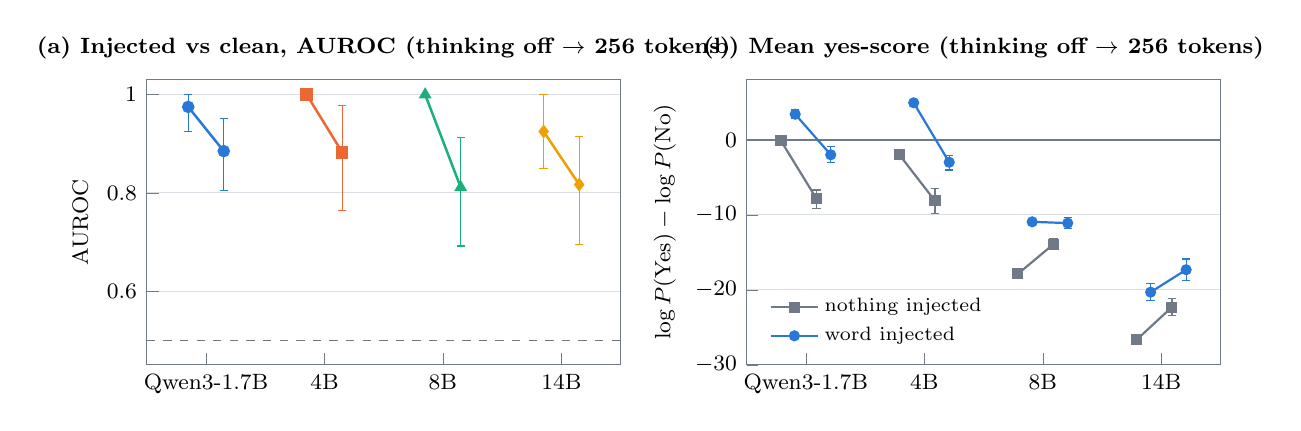
\begin{tikzpicture}
\begin{groupplot}[group style={group size=2 by 1, horizontal sep=1.6cm}, width=7.6cm, height=5.2cm, xtick={1,2,3,4}, xticklabels={Qwen3-1.7B,4B,8B,14B}, xmin=0.5, xmax=4.5]
\nextgroupplot[title={(a) Injected vs clean, AUROC (thinking off $\to$ 256 tokens)}, ymin=0.45, ymax=1.03, ylabel={AUROC}]
\draw[cGrey, dashed, line width=0.5pt] (axis cs:0.5,0.5) -- (axis cs:4.5,0.5);
\addplot[color=cA, mark=*, mark size=1.8pt, line width=0.9pt, err] coordinates {(0.8500,0.97500) += (0,0.02500) -= (0,0.05000) (1.1500,0.88500) += (0,0.06719) -= (0,0.08063)};
\addplot[color=cB, mark=square*, mark size=1.8pt, line width=0.9pt, err] coordinates {(1.8500,1.00000) += (0,0.00000) -= (0,0.00000) (2.1500,0.88250) += (0,0.09625) -= (0,0.11750)};
\addplot[color=cC, mark=triangle*, mark size=1.8pt, line width=0.9pt, err] coordinates {(2.8500,1.00000) += (0,0.00000) -= (0,0.00000) (3.1500,0.81125) += (0,0.10125) -= (0,0.11938)};
\addplot[color=cD, mark=diamond*, mark size=1.8pt, line width=0.9pt, err] coordinates {(3.8500,0.92500) += (0,0.07500) -= (0,0.07500) (4.1500,0.81688) += (0,0.09875) -= (0,0.12125)};
\nextgroupplot[title={(b) Mean yes-score (thinking off $\to$ 256 tokens)}, ymin=-30, ymax=8, ylabel={$\log P(\mathrm{Yes})-\log P(\mathrm{No})$},
  legend pos=south west, legend cell align=left]
\draw[cGrey, line width=0.5pt] (axis cs:0.5,0) -- (axis cs:4.5,0);
\addplot[color=cGrey, mark=square*, mark size=1.6pt, line width=0.8pt, err] coordinates {(0.7900,-0.12500) += (0,0.00000) -= (0,0.00000) (1.0900,-7.85469) += (0,1.16406) -= (0,1.31875)};\addlegendentry{nothing injected}
\addplot[color=cA, mark=*, mark size=1.6pt, line width=0.8pt, err] coordinates {(0.9100,3.41875) += (0,0.56250) -= (0,0.57500) (1.2100,-1.98750) += (0,1.10625) -= (0,1.05781)};\addlegendentry{word injected}
\addplot[color=cGrey, mark=square*, mark size=1.6pt, line width=0.8pt, err, forget plot] coordinates {(1.7900,-2.00000) += (0,0.00000) -= (0,0.00000) (2.0900,-8.13750) += (0,1.63438) -= (0,1.69687)};
\addplot[color=cA, mark=*, mark size=1.6pt, line width=0.8pt, err, forget plot] coordinates {(1.9100,4.94375) += (0,0.48125) -= (0,0.48750) (2.2100,-2.98750) += (0,0.87500) -= (0,1.03438)};
\addplot[color=cGrey, mark=square*, mark size=1.6pt, line width=0.8pt, err, forget plot] coordinates {(2.7900,-17.87500) += (0,0.00000) -= (0,0.00000) (3.0900,-13.91250) += (0,0.80000) -= (0,0.76875)};
\addplot[color=cA, mark=*, mark size=1.6pt, line width=0.8pt, err, forget plot] coordinates {(2.9100,-10.93125) += (0,0.23438) -= (0,0.25625) (3.2100,-11.10156) += (0,0.74219) -= (0,0.74062)};
\addplot[color=cGrey, mark=square*, mark size=1.6pt, line width=0.8pt, err, forget plot] coordinates {(3.7900,-26.68750) += (0,0.00000) -= (0,0.00000) (4.0900,-22.30000) += (0,1.16250) -= (0,1.07812)};
\addplot[color=cA, mark=*, mark size=1.6pt, line width=0.8pt, err, forget plot] coordinates {(3.9100,-20.31406) += (0,1.18594) -= (0,1.13438) (4.2100,-17.32031) += (0,1.42812) -= (0,1.44844)};
\end{groupplot}
\end{tikzpicture}
\end{document}
